
\medskip 

%Pour occuper son petit frère, Lucie, qui aime bien l'informatique, décide de fabriquer des rosaces à colorier. Elle décide de partir d'un motif ayant la forme d'un losange. 
%
%A l'aide d'un logiciel de programmation assisté (type scratch), elle a représenté le motif suivant : 
%
%\begin{center}
%\psset{unit=1cm}
%\begin{pspicture}(10,3.5)
%\pspolygon(1.2,2.7)(5.5,2.7)(9.2,0.6)(4.9,0.6)
%\psarc(1.2,2.7){0.4}{-30}{0}\rput(2.2,2.4){30\degres}
%\psarc(5.5,2.7){0.4}{-180}{-30}\rput(5.1,2.){150\degres}
%\psline[linestyle=dashed](9.2,0.4)(4.9,0.4)\uput[d](7.05,0.4){50}
%\psline(3.45,2.8)(3.45,2.6)\psline(7.05,0.7)(7.05,0.5)
%\psline(3.2,1.4)(3.4,1.7)\psline(7.4,1.4)(7.6,1.7)
%\rput(0.7,2.7){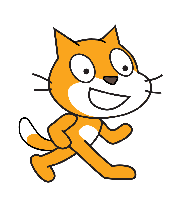
\includegraphics[width=0.8cm]{chat}}
%\end{pspicture}
%\end{center}
%
%%Il s'agit d'un losange dont les côtés ont pour longueur 50 pixels et dont les angles aigus mesurent 30\degres et les angles obtus 150\degres. 
%
%\smallskip
%
%Afin de représenter ce losange, elle a écrit le programme suivant:
 
%\begin{center}
%\parbox{0.4\linewidth}{
%\begin{scratch}
%\blockinit{Quand \greenflag est cliqué}
%\blockpen{effacer tout}
%\blocklook{montrer}
%\blockmove{s'orienter à \ovalnum{90} }
%\blockmove{aller à x: \ovalnum0 y: \ovalnum0}
%\blockvariable{mettre \ovalvariable{Côté} à \ovaloperator{\ldots}}
%\blockmove{Losange}
%\end{scratch}}\hfill
%\parbox{0.4\linewidth}{
%\begin{scratch}
%\initmoreblocks{définir \namemoreblocks{Losange}}
%\blockpen{stylo en position d'écriture}
%\blockrepeat{répéter \ovalnum{2} fois}
%{
%\blockmove{avancer de \ovalnum{Côté}}
%\blockmove{tourner \turnright{} de \ovalnum{\ldots} degrés}
%\blockmove{avancer de \ovalnum{Côté}}
%\blockmove{tourner \turnright{} de \ovalnum{\ldots} degrés}
%}
%\end{scratch}}
%\end{center}

\smallskip

\begin{enumerate}
\item %Compléter dans l'annexe jointe le programme ci-dessus en remplaçant les pointillés par les bonnes valeurs pour que le losange soit dessiné tel qu'il est défini.
Voir l'annexe. 
\item %En utilisant le losange ci-dessus, elle obtient la rosace suivante qui n'est pas en vraie grandeur: 


%\begin{center}
%\psset{unit=1cm}
%\begin{pspicture}(-2,-2)(2,2)
%\def\losange{\pspolygon(0,0)(1,0)(1.866,0.5)(1;30)}
%\multido{\n=0+30}{12}{\rput{\n}(0,0){\losange}}
%\end{pspicture}
%\end{center}
%
%\smallskip

%Quelle transformation géométrique, partant du premier losange ABCD et répétée 12 fois, a été utilisée pour obtenir cette figure ? Définir le mieux que vous pouvez cette transformation.
La rotation de centre O et d'angle 30\degres{} dans n'importe quel sens  répétée 12 fois permet d'obtenir la rosace à partir du losange. 
\item %Pour finir, Lucie souhaite encore compléter cette rosace de trois façons différentes. Pour cela trois programmes ont été effectués. 

%Recopier sur votre copie le numéro des trois programmes, et pour chacun, la lettre de la figure qui lui est associée. 

%\begin{center}
%\begin{tabularx}{\linewidth}{X X X}
%\parbox{0.32\linewidth}{Programme 1 :
%
%\begin{scratch}
%\blockinit{Quand \greenflag est cliqu\'e}
%\blockpen{effacer tout}
%\blocklook{montrer}
%\blockmove{s'orienter à \ovalnum{90} }
%\blockmove{aller \`a x: \ovalnum0 y: \ovalnum0}
%\blockvariable{mettre \ovalvariable{Côt\'e} à \ovaloperator{50}}
%\blockrepeat{répéter \ovalnum{12} fois}
%{\blockevent{Losange}
%\blockmove{tourner \turnright{} de \ovalnum{30} degr\'es}
%}
%\blockmove{ajouter à \ovalvariable{Côt\'e}  \ovaloperator{- 25}}
%\blockrepeat{répéter \ovalnum{12} fois}
%{\blockevent{Losange}
%\blockmove{tourner \turnright{} de \ovalnum{30} degr\'es}
%}
%\blockmove{cacher}
%\end{scratch}}\hfill 
%\parbox{0.32\linewidth}{ Programme 2 :
% 
%\begin{scratch}
%\blockinit{Quand \greenflag est cliqué}
%\blockpen{effacer tout}
%\blocklook{montrer}
%\blockmove{s'orienter à \ovalnum{90} }
%\blockmove{aller à x: \ovalnum0 y: \ovalnum0}
%\blockvariable{mettre \ovalvariable{Côté} à \ovaloperator{50}}
%\blockrepeat{répéter \ovalnum{12} fois}
%{\blockevent{Losange}
%\blockmove{tourner \turnright{} de \ovalnum{30} degrés}}
%\blockmove{tourner \turnright{} de \ovalnum{15} degrés}
%\blockmove{ajouter à \ovalvariable{Côté}  \ovaloperator{10}}
%\blockrepeat{répéter \ovalnum{12} fois}
%{\blockevent{Losange}
%\blockmove{tourner \turnright{} de \ovalnum{30} degrés}
%}
%\blockmove{cacher}
%\end{scratch}}
%\hfill \parbox{0.32\linewidth}{Programme 3 :
%
%\begin{scratch}
%\blockinit{Quand \greenflag est cliqué}
%\blockpen{effacer tout}
%\blocklook{montrer}
%\blockmove{s'orienter à \ovalnum{90} }
%\blockmove{aller à x: \ovalnum0 y: \ovalnum0}
%\blockvariable{mettre \ovalvariable{Côté} à \ovaloperator{50}}
%\blockrepeat{répéter \ovalnum{12} fois}
%{\blockevent{Losange}
%\blockmove{tourner \turnright{} de \ovalnum{30} degrés}}
%\blockmove{ajouter à \ovalvariable{Côté}  \ovaloperator{10}}
%\blockrepeat{répéter \ovalnum{12} fois}
%{\blockevent{Losange}
%\blockmove{tourner \turnright{} de \ovalnum{30} degrés}
%}
%\blockmove{cacher}
%\end{scratch}}

%\end{tabularx}
%\end{center}

%\parbox{0.32\linewidth}{Figure A: 
%
%\psset{unit=1cm}
%\begin{pspicture}(-2,-2)(2,2)
%\def\losange{\pspolygon(0,0)(1,0)(1.866,0.5)(1;30)}
%\multido{\n=0+30}{12}{\rput{\n}(0,0){\losange}}
%\rput{-30}(0,0){\pspolygon[fillstyle=solid,fillcolor=lightgray](0,0)(1,0)(1.866,0.5)(1;30)}
%\psset{unit=1.1cm}
%\def\losange{\pspolygon(0,0)(1,0)(1.866,0.5)(1;30)}
%\multido{\n=0+30}{12}{\rput{\n}(0,0){\losange}}
%
%\end{pspicture}}\hfill
%\parbox{0.32\linewidth}{Figure B : 
%
%\psset{unit=1cm}
%\begin{pspicture}(-2,-2)(2,2)
%\def\losange{\pspolygon(0,0)(1,0)(1.866,0.5)(1;30)}
%\multido{\n=0+30}{12}{\rput{\n}(0,0){\losange}}
%\rput{-30}(0,0){\pspolygon[fillstyle=solid,fillcolor=lightgray](0,0)(1,0)(1.866,0.5)(1;30)}
%\psset{unit=0.5cm}
%\def\losange{\pspolygon(0,0)(1,0)(1.866,0.5)(1;30)}
%\multido{\n=0+30}{12}{\rput{\n}(0,0){\losange}}
%\end{pspicture}}\hfill
%\parbox{0.32\linewidth}{Figure C : 
%
%\psset{unit=1cm}
%\begin{pspicture}(-2,-2)(2,2)
%\def\losange{\pspolygon(0,0)(1,0)(1.866,0.5)(1;30)}
%\multido{\n=0+30}{12}{\rput{\n}(0,0){\losange}}
%\rput{-30}(0,0){\pspolygon[fillstyle=solid,fillcolor=lightgray](0,0)(1,0)(1.866,0.5)(1;30)}
%\psset{unit=1.1cm}
%\def\losange{\pspolygon(0,0)(1,0)(1.866,0.5)(1;30)}
%\multido{\n=-15+30}{12}{\rput{\n}(0,0){\losange}}
%\end{pspicture}
%}
%
%\begin{center}
%Pour plus de lisibilité, le losange initial a été grisé.\end{center} 
Le programme 1 permet d'obtenir la figure B.

Le programme 2 permet d'obtenir la figure C.

Le programme 3 permet d'obtenir la figure A.
\end{enumerate}

\begin{center}\textbf{\large ANNEXE}

\vspace{1cm} 

\textbf{À DÉTACHER DU SUJET ET À JOINDRE AVEC VOTRE COPIE }
\end{center}


\bigskip

\textbf{Question 1 }

\medskip

Compléter le programme ci-dessous en remplaçant les pointillés par les bonnes valeurs pour que le losange soit dessiné tel qu'il est défini. 

\begin{center}
\parbox{0.4\linewidth}{
\begin{scratch}
\blockinit{Quand \greenflag est cliqu\'e}
\blockpen{effacer tout}
\blocklook{montrer}
\blockmove{s'orienter à \ovalnum{90} }
\blockmove{aller \`a x: \ovalnum0 y: \ovalnum0}
\blockvariable{mettre \ovalvariable{C\^ot\'e} à \ovaloperator{\red 50}}
\blockmove{Losange}
\blockmove{Cacher}
\end{scratch}
}\hfill
\parbox{0.4\linewidth}{
\begin{scratch}
\initmoreblocks{d\'efinir \namemoreblocks{Losange}}
\blockpen{stylo en position d'\'ecriture}
\blockrepeat{r\'ep\'eter \ovalnum{2} fois}
{
\blockmove{avancer de \ovalnum{C\^ot\'e}}
\blockmove{tourner \turnright{} de \ovalnum{\red 30} degr\'es}
\blockmove{avancer de \ovalnum{C\^ot\'e}}
\blockmove{tourner \turnright{} de \ovalnum{\red 150} degr\'es}
}
\end{scratch}
}
\end{center}

\vspace{0.5cm}

